% Template for PLoS
% Version 1.0 January 2009
%
% To compile to pdf, run:
% latex plos.template
% bibtex plos.template
% latex plos.template
% latex plos.template
% dvipdf plos.template

\documentclass[10pt]{article}

% amsmath package, useful for mathematical formulas
\usepackage{amsmath}
% amssymb package, useful for mathematical symbols
\usepackage{amssymb}

% graphicx package, useful for including eps and pdf graphics
% include graphics with the command \includegraphics
\usepackage{graphicx}

% cite package, to clean up citations in the main text. Do not remove.
\usepackage{cite}

\usepackage{color} 

% Use doublespacing - comment out for single spacing
\usepackage{setspace} 
\doublespacing

\usepackage{multirow}

% Text layout
\topmargin 0.0cm
\oddsidemargin 0.5cm
\evensidemargin 0.5cm
\textwidth 16cm 
\textheight 21cm

% Bold the 'Figure #' in the caption and separate it with a period
% Captions will be left justified
\usepackage[labelfont=bf,labelsep=period,justification=raggedright]{caption}

% Use the PLoS provided bibtex style
\bibliographystyle{plos2009}

% Remove brackets from numbering in List of References
\makeatletter
\renewcommand{\@biblabel}[1]{\quad#1.}
\makeatother


% Leave date blank
\date{}

\pagestyle{myheadings}
%% ** EDIT HERE **


%% ** EDIT HERE **
%% PLEASE INCLUDE ALL MACROS BELOW

%% END MACROS SECTION

\begin{document}

% Title must be 150 characters or less
\begin{flushleft}
{\Large
\textbf{RNA-Seq Assembly Discovers Many Splice Variants}
}
% Insert Author names, affiliations and corresponding author email.
\\
Likit Preeyanon$^{1}$, 
Jerry B. Dodgson$^{1}$
Hans Cheng$^{2}$, 
C. Titus Brown$^{3,1 \ast}$
\\
\bf{1} Microbiology and Molecular Genetics, Michigan State University, East Lansing, MI, USA.
\\
\bf{2} Avian Disease and Oncology Laboratory, East Lansing, MI, USA.
\\
\bf{3} Department of Computer Science and Engineering, Michigan State University, East Lansing, MI, USA.
\\
$\ast$ E-mail: ctb@msu.edu
\end{flushleft}

% Please keep the abstract between 250 and 300 words
\section*{Abstract}
Comparison of spliced reads and reference gene annotations has been successfully used to discover alternative
splicing in model organisms. However, the method cannot be applied in organisms without high-quality reference genome and
gene annotations. In this article, we introduce a pipeline, based on \emph{de novo} assembly, that constructs gene models with splice
variants.
The pipeline includes a new technique called local assembly that enhances the sensitivity of
alternative splicing detection.
We demonstrates that the pipeline detects many novel splice variants in RNA-Seq data from chicken spleens.
Some of those splice variants; however, only detected by our pipeline and not Cufflinks.
This indicates that the pipeline can be used to facilitate splice variants detection from RNA-Seq.
% Please keep the Author Summary between 150 and 200 words
% Use first person. PLoS ONE authors please skip this step. 
% Author Summary not valid for PLoS ONE submissions.   
\section*{Author Summary}

\section*{Introduction}
Until recently, studies of alternative splicing had been limited to a small number of genes and isoforms due to high-cost and low-throughput sequencing of expressed sequence tags (ESTs) and full-length cDNA libraries.  
RNA sequencing (RNA-Seq) using the next-generation sequencing (NGS) has been used successfully in many studies to gain unprecedented insight into a complexity of transcriptomes.
Novel isoforms have been identified based on reads mapped across known splice junctions or putative splice junctions from annotations.
It has been estimated that, in human, $92-94$\% of multiexon genes undergo alternative splicing and different isoforms are expressed in different tissues\cite{Wang:2008ea}.
This suggests that even in human a large number of splice variants have not been explored.

Sequences from RNA-Seq are very short (~75--250bp for Illumina reads); therefore, it is not feasible to assess gene
and isoform expression without mapping reads to a reference annotation or construct a full-length transcript from
\emph{de novo} assembly.
Several softwares employing different approaches have been developed to reconstruct transcripts from short reads.
Tophat\cite{Trapnell:2009dp} maps reads to a reference genome to identify exons and splice sites \emph{ab initio}.
It first searches for known splie sites in a genome and then tries to map reads across splice juntions to identify exon junctions.
Exon junctions can be used to build gene models by Cufflinks\cite{Trapnell:2010kd}.
On the other hand, Trinity\cite{Grabherr:2011jb}, has been developed to assemble short reads \emph{de novo} to construct transcripts.
Trans-Abyss\cite{Robertson:2010ih} and Oases\cite{Schulz:2012je} are an extension of Abyss\cite{Simpson:2009iv} and Velvet\cite{Zerbino:2008vu,Zerbino:2009jp} assembler that are designed to work with RNA-Seq data.
These programs are comparable at identifying alternative splicing with a slightly different sensitivity and specificity.
However, Oases with Oases-M has been shown to be superior than other \emph{de novo} assembler at discovering isoforms in human and mouse\cite{Schulz:2012je}.

In this study, we present a pipeline that uses Velvet and Oases assembler to discover alternative splicing in RNA-Seq data from chickens.
We use a new technique called a local assembly that enhances sensitivity of alternative splicing detection of Oases.
The results show that the pipeline can detect more isoforms than Oases-M and can detect isoforms not found by
Cufflinks.

% Results and Discussion can be combined.
\section*{Results}


\subsection*{Transcripts from Global and Local Assembly}

Without high-quality annotations, it is necessary to construct gene models with putative isoforms to identify alternative splicing in our samples.
We used Velvet\cite{Zerbino:2008vu} and Oases\cite{Schulz:2012je} assembler to construct transcripts from short reads.
We ran Velvet using default settings except a hash length or k-mer length, which has no default values.
It has been shown that transcripts from a combination of multiple k-mer lengths is superior than a single k-mer
length\cite{Schulz:2012je}.
In addition, we found that different k-mer lengths detected different isoforms from the same dataset
(Fig.~\ref{kmer-variance}).
For that reason, it is necessary to cover a wide range of k-mers to discover as many isoforms as possible.
For this study, we selected a range of kmers from $21-31$ since we found that k-mers outside this range are prone
to introduce assembly errors.

\subsection*{Local Assembly Enhances Isoform Detection}

Performing assembly with multiple k-mers is time and memory consuming.
To facilitate this, we partitioned reads into groups based on their alignments to the chicken genome.
We refer to this method as a local assembly and a conventional assembly method as a global assembly in this study (see materials and methods).
The advantages of the local assembly method is that each group of reads can be assembled using small amount of memory and it can be assembled on different computers.
Unexpectedly, we also found that local assembly detected alternative isoforms not found in global assembly.
As a result, we merged transcripts from both global and local assembly from multiple k-mers to obtain all possible alternative isoforms from our samples.
Figure~\ref{global_vs_local} shows an example of different isoforms detected from two assembly methods.

Using global and local assembly methods, we obtained the different number of contigs.
Table~\ref{unique_sequences} shows the number of contigs from four datasets and unique contigs from global and local assemblies.
As expected, some sequences from local assembly (1,690--2,751) are not found in global assembly.
Homology search in mouse proteins showed that 32--38\% of long unique regions ($>300$ bp) from local assembly match protein
coding sequences (Table~\ref{unique_sequences_matched_mouse}).
This suggests that some isoforms will be missing in the gene models based solely on global assembly.
In addition, a significant number of transcripts from global assembly are unique, which indicates that
approximately at least 3\% of coding sequences are missing in a current chicken genome (sequences not found in local assembly).

\subsection*{Transcripts from Oases-M contain fewer splice junctions}
Transcripts from multiple k-mer lengths can be merged using Oases-M.
It has been demonstrated that merged transcripts are more complete than those from any single kmer length\cite{Schulz:2012je}.
However, sensitivity of Oases-M in detecting alternative isoforms has not been fully evaluated.
To evaluate this, we compared transcripts from global assembly with k-mer lenght from 21--31 and merged transcripts from Oases-M using k-mer=27. We used alignments of ESTs as a control.
The results show that Oases-M detect fewer splice junctions than unmerged global assembly.
The number of total splice junctions and unique splice junctions detected by Oases-M and unmerged assembly is
shown in Table~\ref{Oases-M}.
Only 447 unique splice junctions from Oases-M are supported by ESTs whereas unmerged assembly detects 1,640
unique splice junctions that also found in ESTs.
This suggests that some genuine splice junctions are missing from merging transcripts from multiple k-mer
lengths with Oases-M; therefore, we did not use Oases-M in our pipeline.

\subsection*{Gene models prediction using Gimme}

We developed a program called, Gimme, to constructs a gene model from alignments of transcripts to the genome.
The program can merge all transcripts from multiple-kmers and predict a structure of full-length isoforms and genes.
As shown in figure~\ref{model_comparisons}, our gene models are comparable to other existing gene models.
Total of 14,703 genes were obtained from global assembly and 14,931 genes from local assembly.
However, the number of genes obtained from global + local assembly is only 15,411.
The number of genes and isoforms slightly increased after combining transcripts from global and local
assembly together (Table~\ref{genes_transcripts}). 
This indicates that some transcripts from both methods were merged together.

Most transcripts include a large part of untranslated regions (UTRs), especially $3'$ UTR in our datasets.
These regions are challenging to predict correctly solely from computational methods due to low degree of conservation [?].
RNA-Seq-derived gene models are useful for studying variations within UTR regions, which may be involved in regulation of isoform expression\cite{} (Fig.~\ref{long_utr}).


\subsection*{An overestimated number of genes and transcripts}
The number of genes from our pipeline might be overestimated due to fragmented transcripts.
In our datasets, read coverage is lower at the $5'$ end due to the method used to convert mRNA to cDNA
in library preparation.
A bias of read coverage toward $3'$ end and low expression level result in fragmented transcripts as shown in Fig.~\ref{fragmented_transcripts}.
Moreover, spurious splice junctions due to duplication in genome sequence can lead to a large number of dubious isoforms.
This seems to occur in a few genome sequences such as chromosome E64\_random.
Figure~\ref{isoforms_boxplot} shows that a majority of genes from our gene models have only a few isoforms.

In addition, parameters used in building gene models such as minimum exon/intron size determine how transcripts are merged together, which can increases or decreases the number of isoforms.
In this study, we adjust the parameters to enhance sensitivity of splice junctions detection that may result in overestimation of the number of isoforms.

\subsection*{Validation of Gene Models}

The results show that our pipeline can be used to detect alternative splicing and construct gene models from a large set of transcripts from assembly.
However, many steps in our pipeline can introduce errors to the gene models.
We performed several methods to validate the gene models as described below.

\subsubsection*{Reads Mapped to Gene Models}

Single-end reads from the same datasets that we used to build the gene models were aligned to cDNA sequences derived from the gene models.
We anticipated that a large number of reads could align to the gene models.
We found that 73--78\% of reads mapped to the gene models (Table~\ref{single-end_map}).
In addition, we mapped paired-end reads that we obtained later from the same samples to
the gene models and found that 77--78\% of reads mapped concordantly to the gene models (Table~\ref{paired-end_map}).
The results suggest that the gene models are of high quality.

\subsubsection*{Reads mapped to splice junctions}
To validate the splice junctions, we mapped reads to cDNA sequences derived from gene models using Bowtie\cite{Langmead:2009fv}.
Because the mapping algorithm implemented in Bowtie does not consider splice sites, reads mapped across splice junctions
confirm that the splice junctions are in transcripts.
Of 104,827 splice junctions from the gene models, only 248 (0.23\%) junctions have no spliced reads and 484 (0.46\%)
junctions have 1--3 spliced reads (see materials and methods) (Fig.~\ref{cdf_single_splice}.
The results indicate the method can detect splice junctions with a very high specificity.
Some splice junctions with fewer than four spliced reads; however, may not be false junctions because of a bias of
read coverage toward $3'$ end in our datasets as mentioned earlier.
Reads are less abundant at the $5'$ end of transcripts; consequently, a relatively small number of spliced reads is mapped
to splice junctions near the $5'$ end.

\subsubsection*{Comparison with ESTs and Genbank mRNAs}
82,908 (80.31\%) splice junctions from our gene models are supported by ESTs or Genbank mRNAs.
This illustrates the efficiency of our pipeline in detecting genuine splice junctions.
We also found that 82,750 (99.80\%) junctions that are supported by both Genbank mRNAs and ESTs are also supported by at least four spliced reads.
Therefore, we can assume that splice junctions with more than three spliced reads are likely to be real.
Using this criterion, we can conclude that our gene models include 19,981 novel splice junctions that are not in ESTs and mRNAs.

\subsubsection*{Comparison with Cufflinks}
To evaluate an efficiency of our pipeline in detecting splice junctions,
we compared the number of splice junctions detected by our pipeline to that from Cufflinks\cite{Trapnell:2010kd}, ESTs and
Ensembl gene models version 64.
Cufflinks detected 89,289 (86.49\%) splice junctions that are also detected by our pipeline.
However, 37.61\% (5,565) of junctions not detected by Cufflinks are supported by ESTs.
This suggests that the assembly detects some splice junctions that are not detected by Cufflinks and they are
genuine splice junctions.

We also aligned transcripts from Cufflinks and the pipeline to Ensembl transcripts to compare genes and transcripts detected by
both methods.
We selected only transcripts that match with more than 90\% identity and cover more than 80\% of an Ensembl transcript.
Our pipeline detects 7,046 genes and Cufflinks detects 8,341 genes of total 17,934 Ensembl genes.
6,572 of those genes are both detectd by our pipeline and Cufflinks.
In addition, we wanted to compare the number of isoforms detected by our pipeline and Cufflinks within the same gene; however,
a transcript can match to multiple isoforms in the same gene, especially when it is not complete.
Therefore, we compare the number of splice junctions detected by both methods within the same gene instead.
From 6,572 genes, our pipeline detects 57,437 splice junctions, whereas Cufflinks detects 62,101 junctions.

However, because Ensembl gene models do not include all isoforms or splice junctions from ESTs, we investigated splice junctions
that are not in Ensembl but are supported by ESTs in those 6,572 genes and found that our pipeline detects 2,260 splice junctions
and Cufflinks only detects 1,588 splice junctions. Figure ~\ref{alt_splice_site} shows an example of splice junctions not included in Ensembl gene models, which are detected by our pipeline.

To conclude, Cufflinks performs better than our pipeline for detecting both genes and splice junctions in Ensembl gene models.
However, we found that our pipeline detects more splice junctions that are not in Ensembl but are supported by ESTs.


\subsubsection*{Merged gene models from assembly and Cufflinks}
As shown above, Cufflinks and assembly method detect non-overlapped splice junctions,
which suggests that we should to combine gene models from two methods to
obtain more complete gene models or to detect more splice junctions.
We obtained a total of 16,445 genes with 53,296 transcripts from Cufflinks + assembly gene models.
As shown in Table.~\ref{genes_transcripts}, the number of genes from Cufflinks + assembly gene models
decreases, which indicates that some fragmented transcripts are merged together and form a more complete gene structure (Fig.~\ref{cufflinks_asm}).

\subsubsection*{Homologous sequences in mouse}
Splice variants must maintain the reading frame to be translated to functional proteins.
Based on this assumption, we investigated isoforms in our gene models by searching for homologous protein sequences in
other organism.
To obtain a protein sequence of each isoform, we translated a cDNA sequence using ESTScan\cite{Iseli:1999vd},
which is designed to translate
protein sequences from incomplete cDNA sequences such as ESTs.
ESTScan succesfully translated 42,459 (94.5\%) of all isoforms to protein sequences with 50 or longer amino acids.
Then, all protein sequences were searched for homology in mouse \textit{(Mus musculus)}, which is a related and well-studied animal.
We found 26,931 (63.43\%) isoforms from 4,165 genes match mouse proteins.
As shown in Fig.~\ref{bitscore}, most genes and isoforms have a bit score/length ratio more than 1.0, which
indicates a good agreement between chicken and mouse proteins.
The results illustrate that isoforms constructed by our pipeline are translatable and may be functional.
However, genes or isoforms with no match to mouse proteins are not necessarily artifacts.
They can be genes or isoforms that are only found in non-mammal vertebrates or novel genes.

\section*{Discussion}

Choice of k-mers greatly affects sensitivity of splice variants detection in RNA-Seq assembly using Velvet/Oases.
Short k-mers increase sensitivity, but also introduce errors from misassembly.
However, for a study focusing on alternative splicing, it is desirable to detect as many splice variant as possible.
We have presented the local assembly technique that enhances the ability to detect splice variants of Velvet/Oases from the same
k-mer.
The mechanism behind this technique is to be investigated.
Importantly, understanding of the mechanisms may lead to a filtering technique that can be applied to organisms that lack a reference genome.

We have also developed a pipeline that assembles reconstructed transcripts from multiple k-mers to build putative gene models.
Overall, a majority of splice variants detected by our pipeline are also detected by Cufflinks.
Both our pipeline and Cufflinks also detect some splice variants that are not overlapped.
Combination of both methods results in more complete gene models,
which suggests that combination of \emph{de novo} assembly and reference-based assembly is preferred to study alternative splicing in chicken.

Interestingly, Cufflinks detects more genes and isoforms included in Ensembl annotations than our pipeline.
However, our pipeline detects many more splice junctions not included in Ensembl but supported by ESTs.
As observed in previous study by Schulz \emph{et al.}\cite{Schulz:2012je}, Cufflinks also outperforms \emph{de novo} assembly in
detecting genes and isoforms in Ensembl annotations in mouse.
We speculate that Cufflinks possesses a mechanism that is tailored to detect Ensembl gene models.

In this study, gene models are built from chicken genome version 2.1 (galGal3),
which contains a considerable number of sequence duplications and
missassemblies that supposed to be eliminated in the latest version of genome assembly (galGal4).
Duplications and misassemblies lead to false splice junctions, which in turn produce a large number of splice variants as
observed in some chromosomes.
Conversely, this suggests that one might be able to use the pipeline to evaluate the quality of reference genome.

% You may title this section "Methods" or "Models". 
% "Models" is not a valid title for PLoS ONE authors. However, PLoS ONE
% authors may use "Analysis" 
\section*{Materials and Methods}

\subsection*{Quality trimming of reads}
Both single- and paired-end reads in this study were trimmed using Condetri version 2.1 with default parameters.
In addition, the first 10 bases of each reads were trimmed off due to an inconsistency of base-calling as shown in supplementary figure S?.

\subsection*{Mapping reads to The Reference Genome and Gene Models}

Single and paired-end reads were mapped to chicken genome by Tophat2\cite{Trapnell:2009dp} release 2.0.0 using
default parameters without annotations.
All reads were mapped to cDNA sequences derived from gene models by Bowtie2\cite{Langmead:2009fv} with
default parameters \texttt{(n=2, l=28, e=70, k=1)}.

\subsection*{Global and Local Assembly}

Reads from each dataset were first assembled separately in global assembly without using a reference genome.
In contrast, reads from each dataset were first mapped to the chicken genome using Tophat2.
Then only reads mapped to the genome were assembled by chromosomes in local assembly (Fig.~\ref{local_assembly}).
Global and local assembly was performed using Velvet version 1.2.03\cite{Zerbino:2008vu}
with default parameters except for hash length (k-mer).
A range of k-mer length from 21-31 was used to assemble reads in both global and local assembly.
Lastly, transcripts from both methods were assembled by Oases version 0.2.06\cite{Schulz:2012je}.

A poly-A tail, short transcripts and transcripts with low complexity are removed by
seqclean\cite{seqclean} with default parameters.
Redundant transcripts are removed by cd-hit-est from CD-HIT suite\cite{Li:2006hr}.
A large number of transcripts are removed at this step, which facilitates gene models construction process.

We obtained 334,475 transcripts, of which 295,588 transcripts (88.37\%) mapped to chicken genome.
Only transcripts mapped to chicken genome are used to build gene models.

\subsection*{Gene Model Construction}

\subsubsection*{Overall Pipeline}

Figure~\ref{overall_pipeline} depicts an overall gene model construction pipeline.
Transcripts of all datasets from local and global assembly were mapped to the chicken genome using
BLAT\cite{Kent:2002tv} \texttt{(-t=dna -q=dna -noHead -out=psl -mask=lower -extendThroughN -dots=1000)}.
Alignments and gaps from BLAT outputs are considered exons and introns respectively.
Optionally, data from other sources (ESTs, RefGenes, etc.) can be incorporated with transcripts from assembly to improve gene models.
All transcripts are then assembled using Gimme, a program that assembles transcripts based on their alignments to the reference genome.
An algorithm for assembling transcripts is described below.
A maximum set of transcripts obtained from Gimme are then reduced to only a minimum set of transcripts that contain
all splice junctions and untranslated regions (UTRs).
After that, transcripts that are identical are clustered and removed by CD-HIT version 4.5.6\cite{Li:2006hr}.
Parameters for clustering are \texttt{-n 10, -r 0 and -c 1.0}.
Only a representative of each cluster is kept in gene models.

\subsubsection*{Algorithm}

A gene model can be represented as a splice graph composed of exons as nodes and introns as edges.
However, transcripts of the same gene vary in size and structure depending on the expression level and a hash length number used in assembly.
Furthermore, incomplete exons and fragmented transcripts complicate the construction of a splice graph.
In this study, we developed an algorithm that handles incomplete exons and fragmented transcripts and constructs a maximum assembly of gene models.

The algorithm first builds an intron graph using introns as nodes.
Each intron contains exons whose one of their splice sites perfectly match intron boundary.
Exons are considered incomplete and eliminated if they locate at the $3'$ or $5'$ end of the transcripts and
they are not the largest exons (exon 3a and 3b in Fig.~\ref{algorithm}).
Transcripts were then grouped into the same gene if they have at least one intron or exon in common.
Then, a splice graph composed of exons is created and structures of isoforms are derived from traversing paths in the splice graph.
Gimme is open-source and available at \texttt{https://github.com/ged-lab/gimme}.

\subsection*{Protein sequence translation}

We employed ESTScan version 2.1 to translate protein sequences from our gene models.
The matrix used for building Hidden Markov model was built from chicken reference cDNA sequences using tools from ESTScan.

\subsection*{Finding unique sequences between datasets}

To identify unique sequences from two datasets, a set of 20-mers is created for both datasets using
khmer\cite{khmer}.
Then, 20-mers from a query dataset are compared with 20-mers from the target dataset.
The sequence is considered unique if more than 90\% of 20-mers in the query is unique.
Any unique region shorter than 100 bp is ignored.

\subsection*{Sequence homology analysis}

Protein sequences translated from each isoform using ESTScan were searched against mouse reference proteins by BLAST 2.2.25+\cite{Tatusova:1999tz}.
A bit score to a length ratio was calculated for each hit that had an e-value $\le 10^{-20}$.
Only the highest value of all isoforms from each gene was shown in the gene plot; whereas, values of all isoforms were shown in the isoform plot.

\subsection*{Spliced reads count}

Reads from each dataset were mapped to transcripts from the gene models using Bowtie version 2.0-beta 5 with default parameters.
Reads mapped across exon junctions from all datasets were counted using Samtools\cite{Li:2009vz} and
Pysam\cite{pysam}

\subsection*{Sequence assembly using Cufflinks}
Reads are mapped to a genome sequence using Tophat2.
Gene models are built from each datasets by Cufflinks 2.0.0\cite{Trapnell:2010kd}.
All gene models are then merged together using Cuffmerge.

\subsection*{Expressed sequence tags and Genbank mRNA}
Expressed sequence tags (ESTs) and mRNAs were downloaded from UCSC genome website on May 9th, 2012.
The database last updated from GENBANK on April 29th, 2012.
Sequences were alignd to a chicken genome using BLAT.

% Do NOT remove this, even if you are not including acknowledgments
%\section*{References}
% The bibtex filename
\bibliography{refs}

\section*{Tables}
\begin{table}[!ht]
\caption{
\bf{Unique sequences from global and local assembly}}
\begin{tabular}{ccccc}
\hline
Dataset & \multicolumn{2}{c}{Total Sequence} & \multicolumn{2}{c}{Unique Sequence}\\
 & Global & Local & Global & Local\\
\hline
Line 6 uninfected & 338,353 & 335,180 & 10,068 (2.97\%) & 1,258 (0.37\%)\\
Line 6 infected & 353,485 & 319,920 & 11,639 (3.29\%)& 2,270 (0.70\%)\\
Line 7 uninfected & 335,876 & 302,443 & 10,649 (3.17\%) & 1,570 (0.51\%)\\
Line 7 infected & 371,404 & 327,491 & 11,859 (3.19?\%)& 1,199 (0.36\%)\\
\hline
%table information
\end{tabular}
%\begin{flushleft}Table Caption
%\end{flushleft}
\label{unique_sequences}

\caption{
\bf{Unique regions from global and local assembly}}
\begin{tabular}{ccccc}
\hline
Dataset & \multicolumn{2}{c}{Unique Region} & \multicolumn{2}{c}{Matched with mouse proteins}\\
 & Global & Local & Global & Local\\
\hline
Line 6 uninfected & 2,132 & 104 & 1,322 (62.01\%) & 39 (37.50\%)\\
Line 6 infected & 2,499 & 104 & 1,514 (60.58\%)& 40 (38.46\%)\\
Line 7 uninfected & 2,633 & 136 & 1,560 (59.25\%) & 52 (38.24\%)\\
Line 7 infected & 2,409 & 152 & 1,390 (57.70\%)& 50 (32.89\%)\\
\hline
%table information
\end{tabular}
%\begin{flushleft}Table Caption
%\end{flushleft}
\label{unique_sequences_matched_mouse}

\caption{
\bf{Number of total and unique splice junctions}}
\begin{tabular}{cccccc}
\hline
Method& Total & Unique & Supported by ESTs \\ 
\hline
Oases-M assembly & 114,336 & 8,735 & 447 (5.1\%) \\
Unmerged assembly & 115,159 & 9,558 & 1,640 (17.15\%) \\
\hline
%table information
\end{tabular}
%\begin{flushleft}\footnotesize \textit{*Minumum set}
%\end{flushleft}
\label{Oases-M}

\caption{
\bf{Number of putative genes and isoforms}}
\begin{tabular}{cccccc}
\hline
Method& Gene & Isoform \\ 
\hline
Global & 14,703 & 28,406 \\
Local & 14,931 & 22,127 \\
Global + Local & 15,411 & 35,598 \\
Cufflinks & 25,318 & 34,959 \\
Global + Local + Cufflinks & 16,445 & 53,296\\
Ensembl & 17,934 & 23,392 \\
\hline
%table information
\end{tabular}
%\begin{flushleft}\footnotesize \textit{*Minumum set}
%\end{flushleft}
\label{genes_transcripts}

\caption{
\bf{Single-end reads mapped to gene models (maximum)}}
\begin{tabular}{cccccc}
\hline
Dataset & Mapped & Unmapped \\
\hline
Line 6 uninfected & 18,398,569 (78.03\%) & 5,180,983 (21.97\%) \\
Line 6 infected & 17,194,894 (73.33\%) & 6,254,087 (26.67\%) \\
Line 7 uninfected & 18,148,112 (75.85\%) & 5,777,697 (24.15\%) \\
Line 7 infected & 19,914,624 (78.52\%) & 5,447,943 (21.48\%) \\
\hline
%table information
\end{tabular}
%\begin{flushleft}Table Caption
%\end{flushleft}
\label{single-end_map}

\caption{
\bf{Paired-end reads mapped to gene models (maximum)}}
\begin{tabular}{cccccc}
\hline
Dataset & Mapped & Unmapped \\
\hline
Line 6 uninfected & 21,641,202 (77.65\%) & 12,022,675 (22.35\%) \\
Line 6 infected & 18,556,277 (77.61\%) & 5,352,216 (22.39\%) \\
Line 7 uninfected & 25,670,333 (77.97\%) & 7,250,999 (22.03\%) \\
Line 7 infected & 26,988,536 (78.27\%) & 7,489,299 (21.73\%) \\
\hline
%table information
\end{tabular}
%\begin{flushleft}Table Caption
%\end{flushleft}
\label{paired-end_map}
\end{table}

\section*{Figure Legends}
\begin{figure}[!ht]
\begin{center}
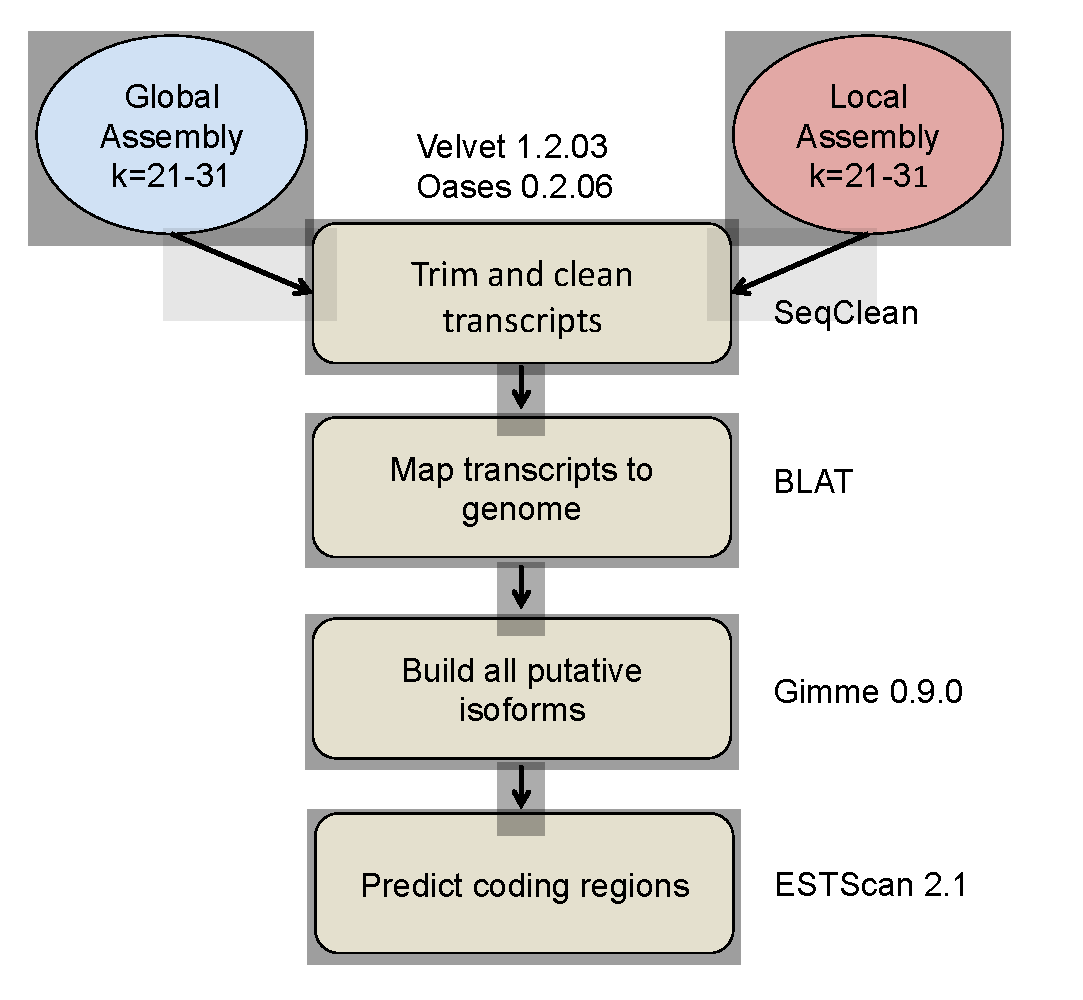
\includegraphics[width=5in]{overall_pipeline.pdf}
\end{center}
\caption{
{\bf Gene model construction pipeline.} Transcripts are obtained from two assembly methods -- global and local assembly.
Transcripts are aligned to a chicken genome by BLAT. Gimme then constructs gene models based on alignments of transcripts.
}
\label{overall_pipeline}
\end{figure}

\begin{figure}[!ht]
\begin{center}
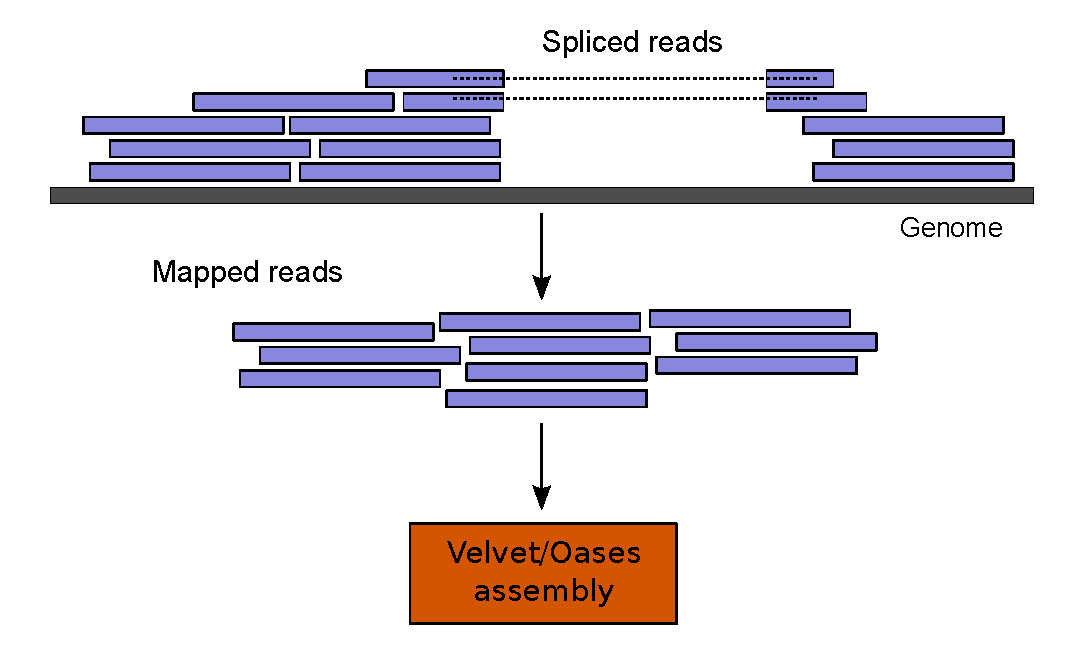
\includegraphics[width=5in]{local_assembly}
\end{center}
\caption{
{\bf Local Assembly Pipeline.}
Reads are first mapped to a chicken genome.
Then only mapped reads are assembled by Velvet and Oases.
}
\label{local_assembly}
\end{figure}

\begin{figure}[!ht]
\begin{center}
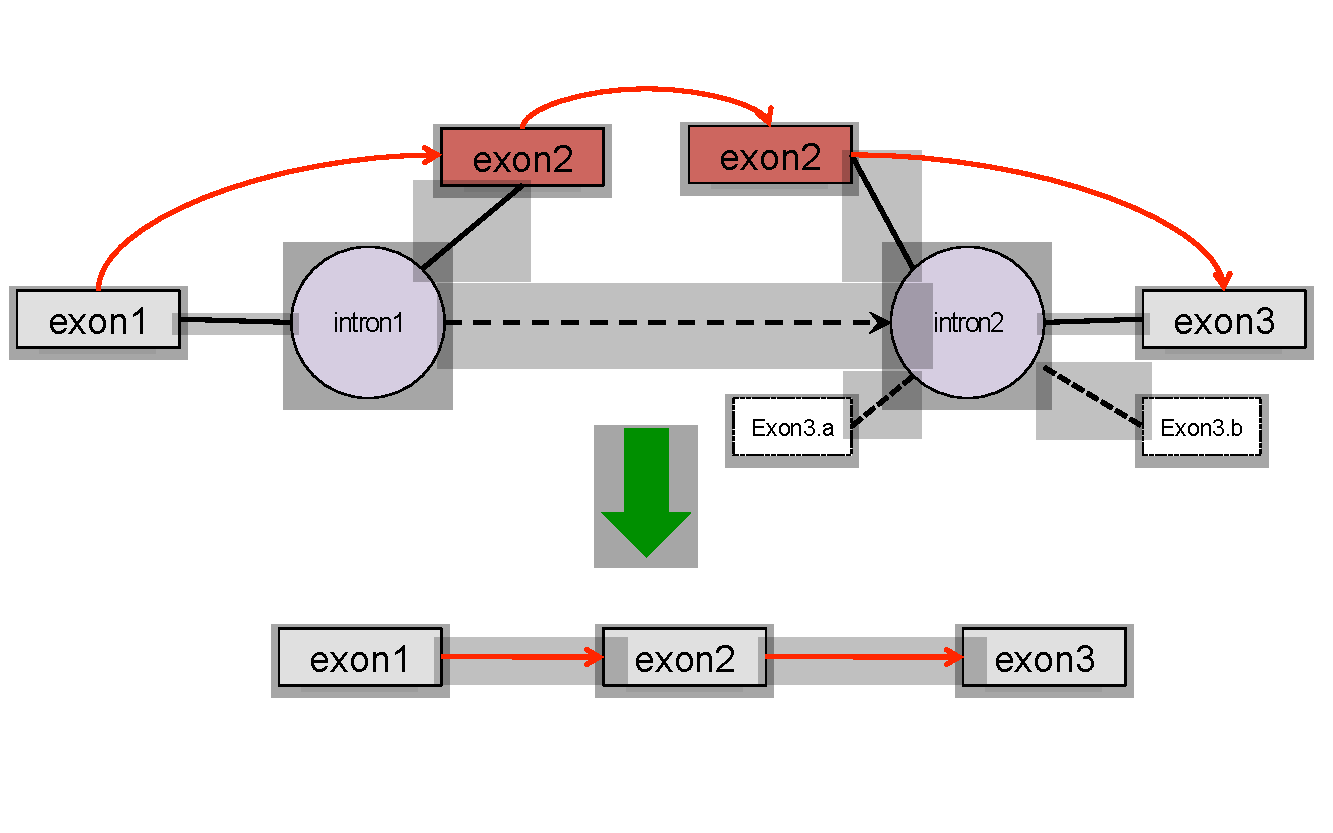
\includegraphics[width=5in]{algorithm.pdf}
\end{center}
\caption{
{\bf Intron and exon graphs.}
Each intron connects to exons whose splice junctions match it boundary.
Some exons are excluded from the final gene model if they are incomplete (exon 3a,b).
Introns sharing at least one exon are grouped together.
Then an exon graph is made using exons as nodes.
}
\label{algorithm}
\end{figure}

\begin{figure}[!ht]
\begin{center}
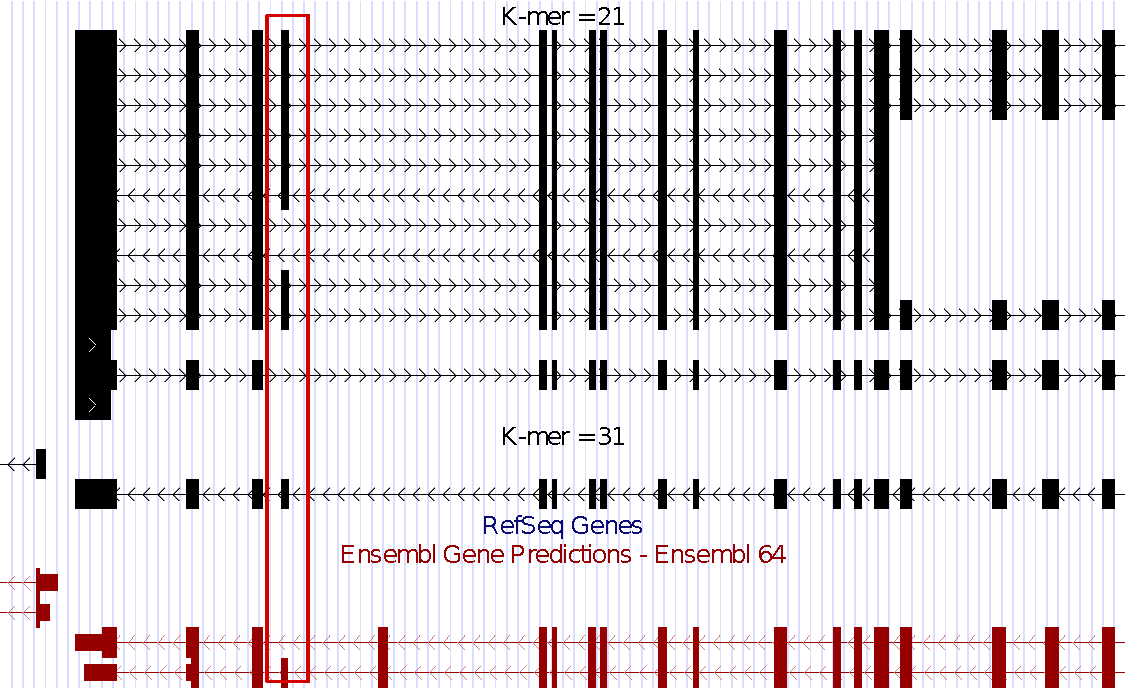
\includegraphics[width=5in]{kmers-variance.pdf}
\end{center}
\caption{
{\bf Different isoforms are detected by different k-mer lengths.}
K-mer=21 detects a skipped exon which is not detected by k-mer=31.
The skipped exon is also annotated in Ensembl gene models.
}
\label{kmer-variance}
\end{figure}

\begin{figure}[!ht]
\begin{center}
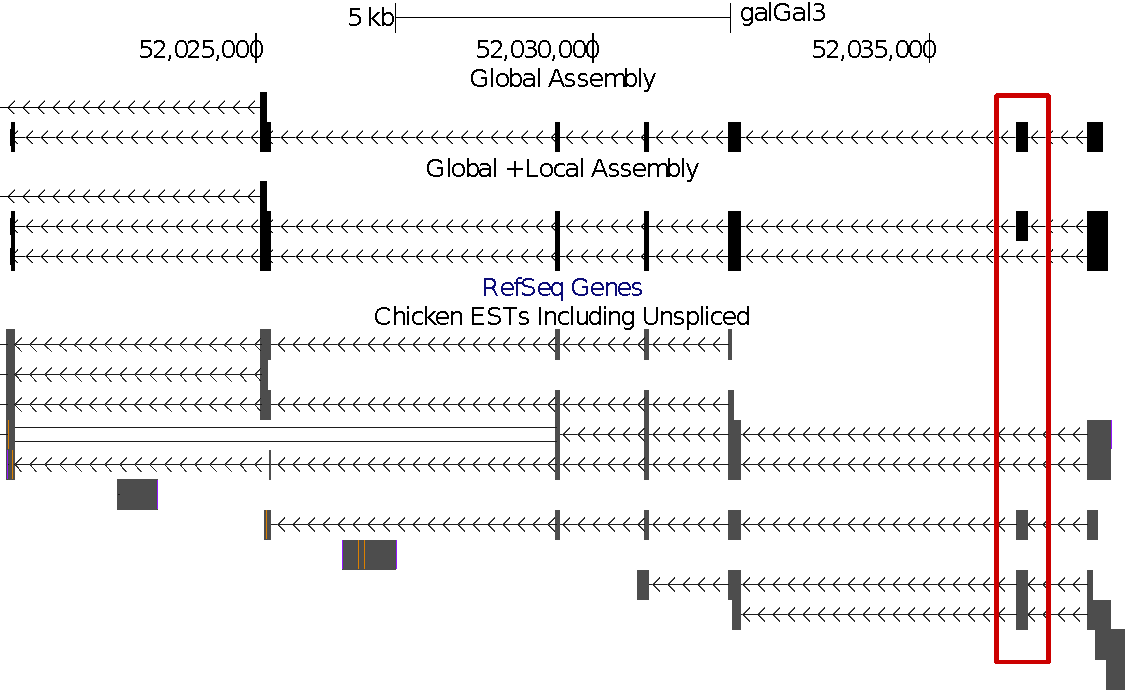
\includegraphics[width=5in]{global_vs_local.pdf}
\end{center}
\caption{
{\bf Global and local assembly detect different isoforms with the same k-mers.} 
}
\label{global_vs_local}
\end{figure}

\begin{figure}[!ht]
\begin{center}
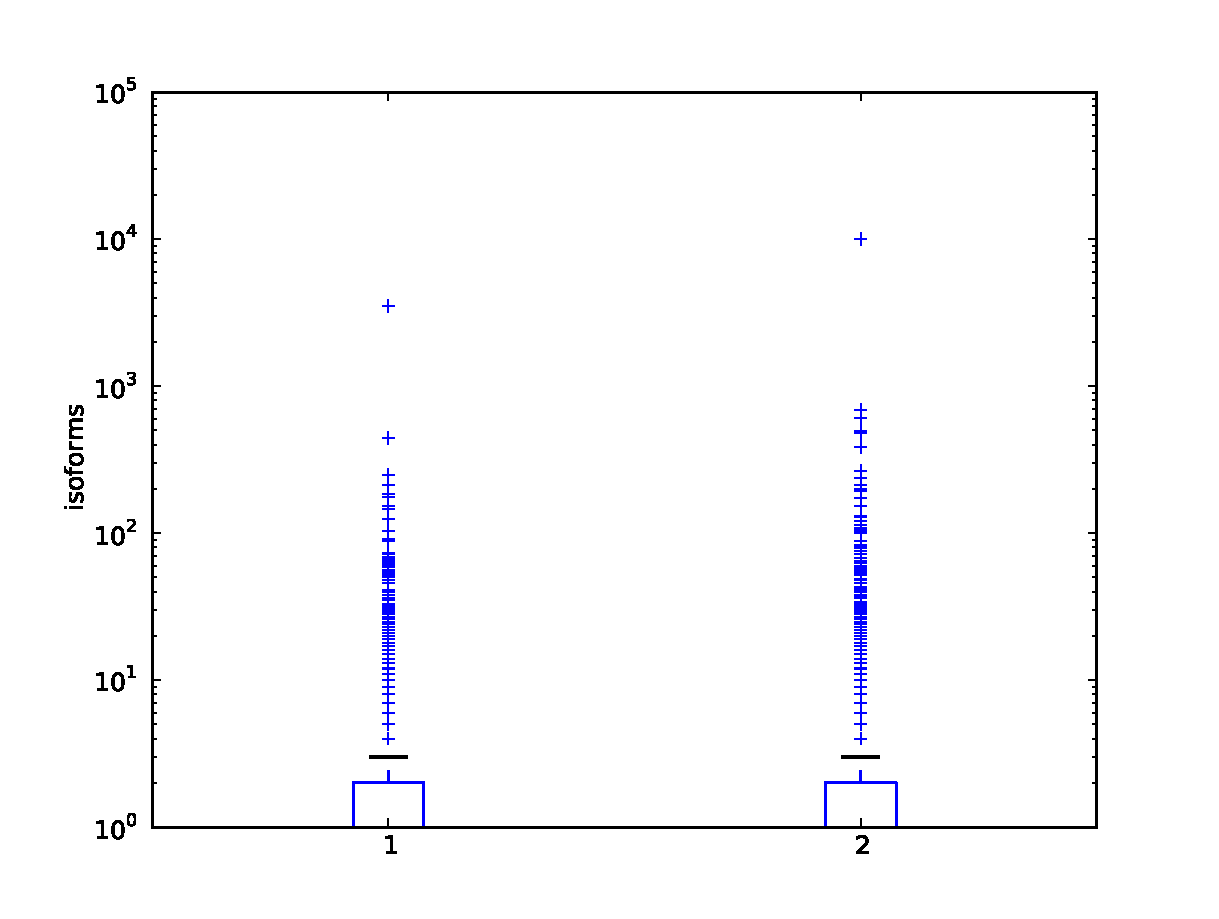
\includegraphics[width=5in]{isoforms_boxplot.pdf}
\end{center}
\caption{
{\bf Distribution of the number of isoforms in each gene from 1) global and 2) local assembly}
}
\label{isoforms_boxplot}
\end{figure}

\begin{figure}[!ht]
\begin{center}
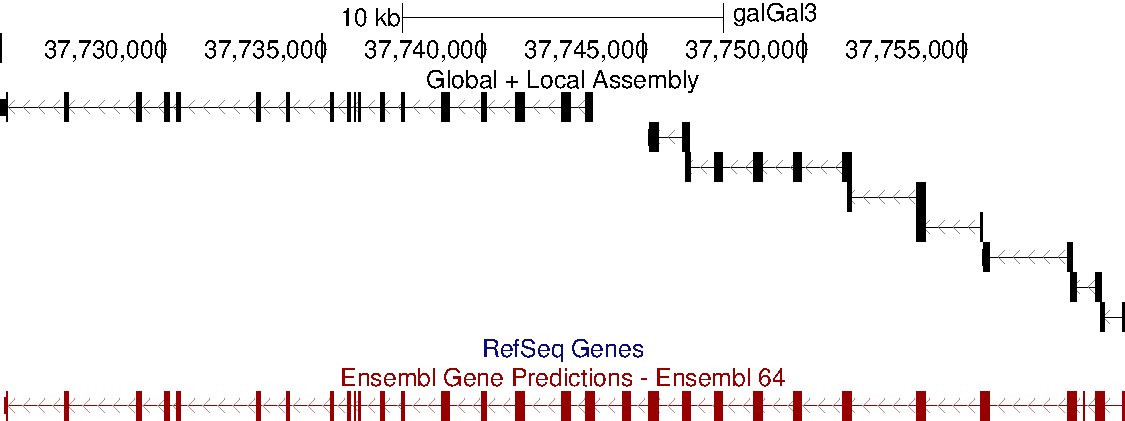
\includegraphics[width=5in]{fragmented_transcripts.pdf}
\end{center}
\caption{
{\bf Example of fragmented transcripts near $5'$ end of a long transcript.}
}
\label{fragmented_transcripts}
\end{figure}

\begin{figure}[!ht]
\begin{center}
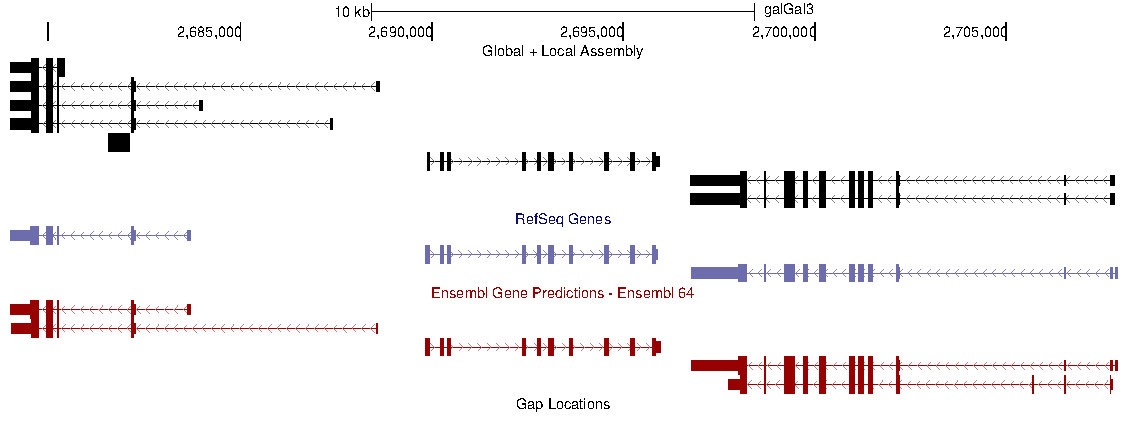
\includegraphics[width=5in]{model_comparisons.pdf}
\end{center}
\caption{
{\bf Comparison of gene models from our pipeline and other public gene models on UCSC genome browser.}
}
\label{model_comparisons}
\end{figure}

\begin{figure}[!ht]
\begin{center}
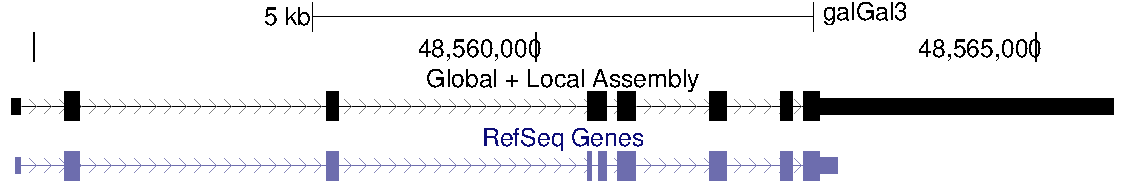
\includegraphics[width=5in]{long_utr.pdf}
\end{center}
\caption{
{\bf Examples of an extended $3'$ UTR detected in RNA-Seq gene models.}
}
\label{long_utr}
\end{figure}

\begin{figure}[!ht]
\begin{center}
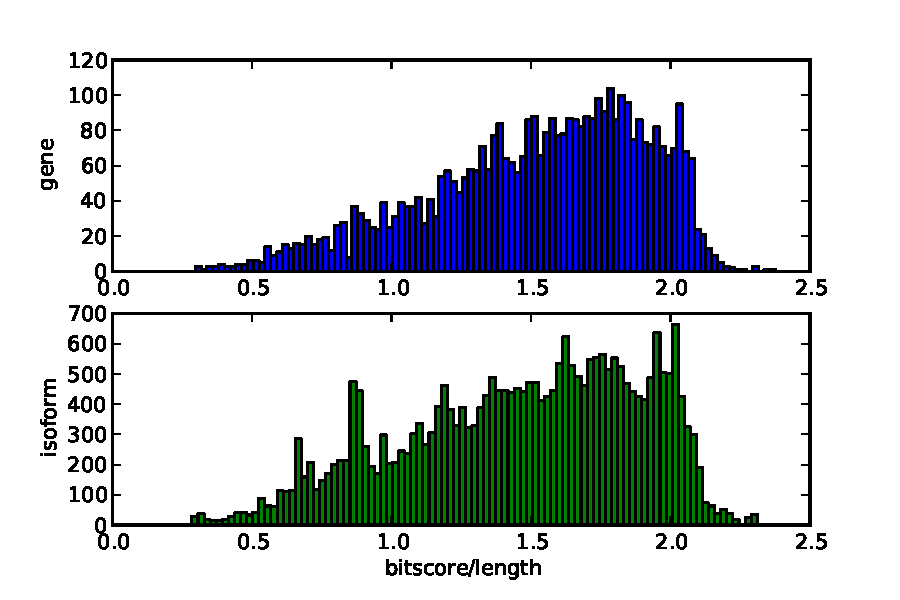
\includegraphics[width=5in]{bitscore.pdf}
\end{center}
\caption{
{\bf Histogram of bit score/length ratio of isoforms and genes that match mouse proteins.}
Genes and isoforms in chromosome E64\_random are not included.
}
\label{bitscore}
\end{figure}

\begin{figure}[!ht]
\begin{center}
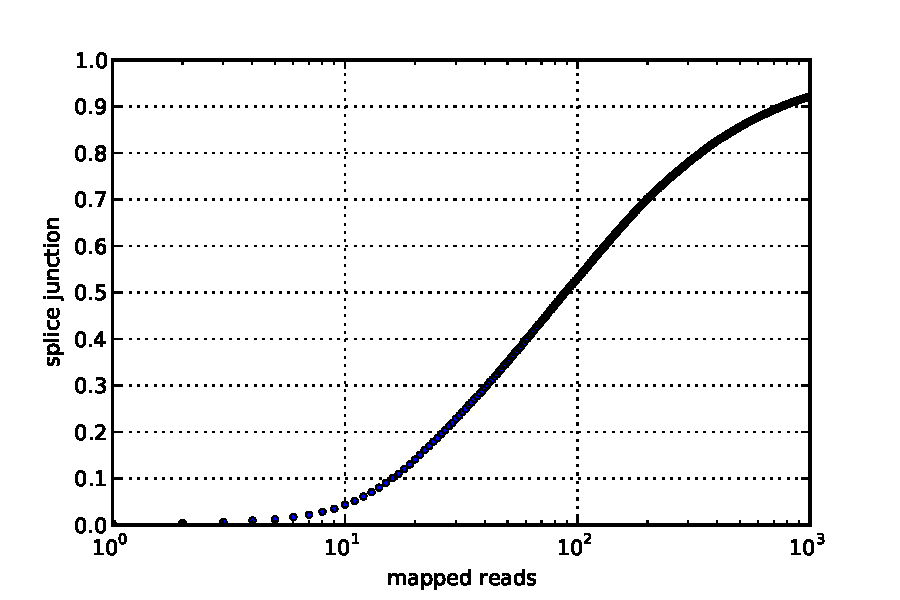
\includegraphics[width=5in]{cdf_single_splice.pdf}
\end{center}
\caption{
{\bf Cumulative counts of splice junctions with spliced reads up to 1000 reads.}
}
\label{cdf_single_splice}
\end{figure}

\begin{figure}[!ht]
\begin{center}
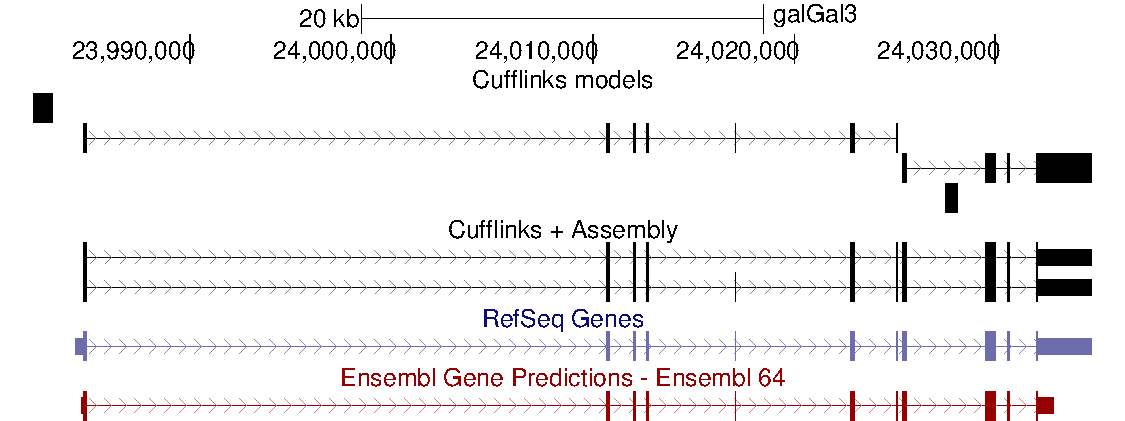
\includegraphics[width=5in]{asm-cufflinks.pdf}
\end{center}
\caption{
{\bf Cufflinks + Assembly gene models.}
Fragmented transcripts in Cufflinks models are merged together after merging with gene models from assembly.
An isoform from assembly that is not in Cufflinks is also added to the gene model.
}
\label{cufflinks_asm}
\end{figure}

\begin{figure}[!ht]
\begin{center}
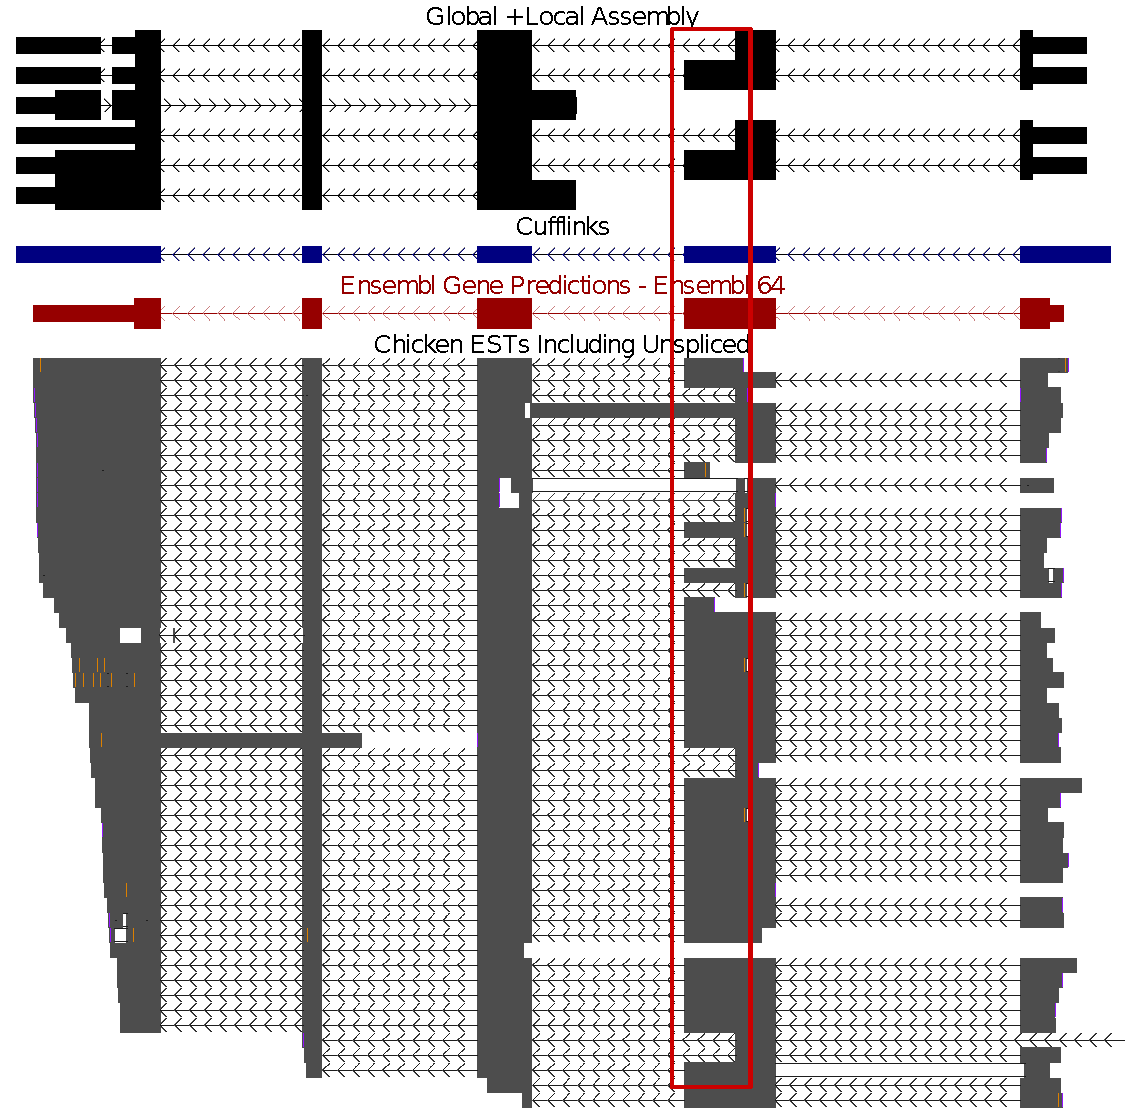
\includegraphics[width=5in]{alt_splice_site.pdf}
\end{center}
\caption{
{\bf Unannotated alternative splice site.}
The pipeline can detect alternative splice site that is not annotated in Ensembl and Cufflinks.
}
\label{alt_splice_site}
\end{figure}

\end{document}
